% Column score from winning splits, toy example (3 splits, 9 columns, k=2).
\definecolor{twcCoral}{HTML}{D85A30}%
\definecolor{twcPurple}{HTML}{7F77DD}%
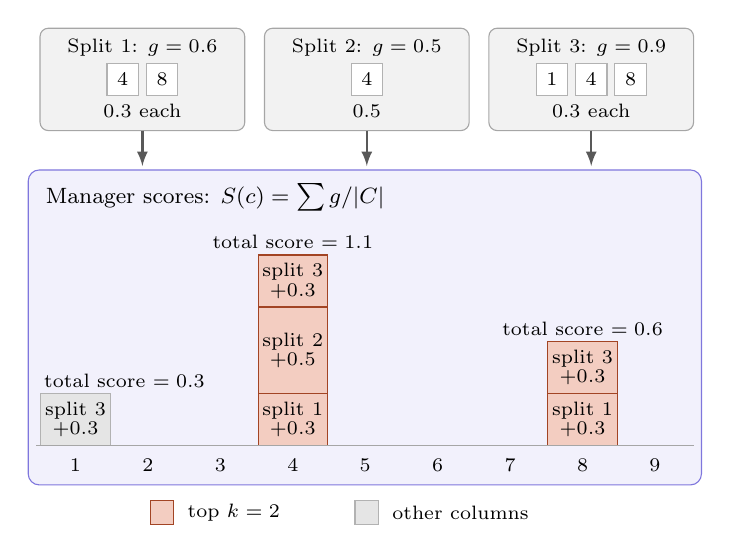
\begin{tikzpicture}[x=1cm,y=1cm,>=latex,
  split/.style={draw=gray!70, fill=gray!10, rounded corners=3pt},
  chip/.style={draw=gray!60, fill=white, minimum size=0.4cm, inner sep=0pt, font=\scriptsize},
  seg/.style={font=\scriptsize, align=center, inner sep=0pt},
  top/.style={draw=twcCoral!75!black, fill=twcCoral!30},
  oth/.style={draw=gray!60, fill=gray!20}]
% winning splits from trees 0..i-1
\foreach \x/\n/\g/\each in {1.35/1/0.6/0.3 each, 4.2/2/0.5/0.5, 7.05/3/0.9/0.3 each} {
  \draw[split] (\x-1.3,4.0) rectangle (\x+1.3,5.3);
  \node[font=\scriptsize] at (\x,5.05) {Split \n: $g=\g$};
  \node[font=\scriptsize] at (\x,4.25) {\each};
  \draw[->, thick, gray!70!black] (\x,4.0) -- (\x,3.55);
}
\node[chip] at (1.1,4.65) {4}; \node[chip] at (1.6,4.65) {8};
\node[chip] at (4.2,4.65) {4};
\node[chip] at (6.55,4.65) {1}; \node[chip] at (7.05,4.65) {4}; \node[chip] at (7.55,4.65) {8};
% manager box holding the per-column scores
\draw[draw=twcPurple, fill=twcPurple!10, rounded corners=4pt] (-0.1,-0.5) rectangle (8.45,3.5);
\node[anchor=north west, font=\footnotesize] at (0.0,3.45) {Manager scores: $S(c)=\sum g/|C|$};
% stacked bars, one segment per split share (1 unit = 2.2cm)
\def\twcseg#1#2#3#4#5#6{\draw[#1] (#2-0.44,#3) rectangle (#2+0.44,#4);
  \node[seg] at (#2,{(#3+#4)/2}) {split #5\\[-1pt]$+#6$};}
\twcseg{oth}{0.5}{0}{0.66}{3}{0.3}
\twcseg{top}{3.26}{0}{0.66}{1}{0.3}
\twcseg{top}{3.26}{0.66}{1.76}{2}{0.5}
\twcseg{top}{3.26}{1.76}{2.42}{3}{0.3}
\twcseg{top}{6.94}{0}{0.66}{1}{0.3}
\twcseg{top}{6.94}{0.66}{1.32}{3}{0.3}
\node[anchor=south west, font=\scriptsize, inner sep=1pt] at (0.06,0.7) {total score $=0.3$};
\node[anchor=south, font=\scriptsize, inner sep=1pt] at (3.26,2.46) {total score $=1.1$};
\node[anchor=south, font=\scriptsize, inner sep=1pt] at (6.94,1.36) {total score $=0.6$};
\draw[gray!70] (0,0) -- (8.35,0);
\foreach \c in {1,...,9} \node[font=\scriptsize] at ({0.5+(\c-1)*0.92},-0.25) {\c};
% legend
\node[top, minimum size=0.3cm, inner sep=0pt] at (1.6,-0.85) {};
\node[anchor=west, font=\scriptsize] at (1.8,-0.85) {top $k=2$};
\node[oth, minimum size=0.3cm, inner sep=0pt] at (4.2,-0.85) {};
\node[anchor=west, font=\scriptsize] at (4.4,-0.85) {other columns};
\end{tikzpicture}
